\chapter{Entropy Drift and the Thermodynamic Cost of Erasure}
\label{chap:entropy_drift}
\includegraphics[width=0.9\textwidth]{images/institutional_fragility_cascade_ch3.png}

\section{Thermodynamic Drift as Political Signal}
\label{sec:thermo_drift_signal}

When I first ran the entropy calculations tied to the Landauer limit, I thought I was only mapping thermodynamic costs. But as I began drawing connections between physical erasure and political erasure, I realized: entropy isn't just an abstract thermodynamic variable—it’s a warning.

\section{Procurement Patterns as Entropy Indicators}
\label{sec:procurement_entropy}

I pulled procurement data from the FPDS database covering DHS, ICE, and associated subcontractors like Palantir and SpaceX-linked vendors. As I tracked line items—personnel, weapons, surveillance tech—I noticed a distinct pattern: entropy dropped year by year. Not just in language. In decisions. In allocations. In intent.

\section{The Political Cost of Erasure}
\label{sec:political_cost_erasure}

The thermodynamic cost of erasure has a political analog: the cost of destroying information, dissent, or complexity in a system. The lower the entropy, the fewer the choices left. And at some point, those choices disappear entirely. That’s what I saw forming—not in theory, but in procurement logs funded by my own government.

\begin{figure}[H]
  \centering
  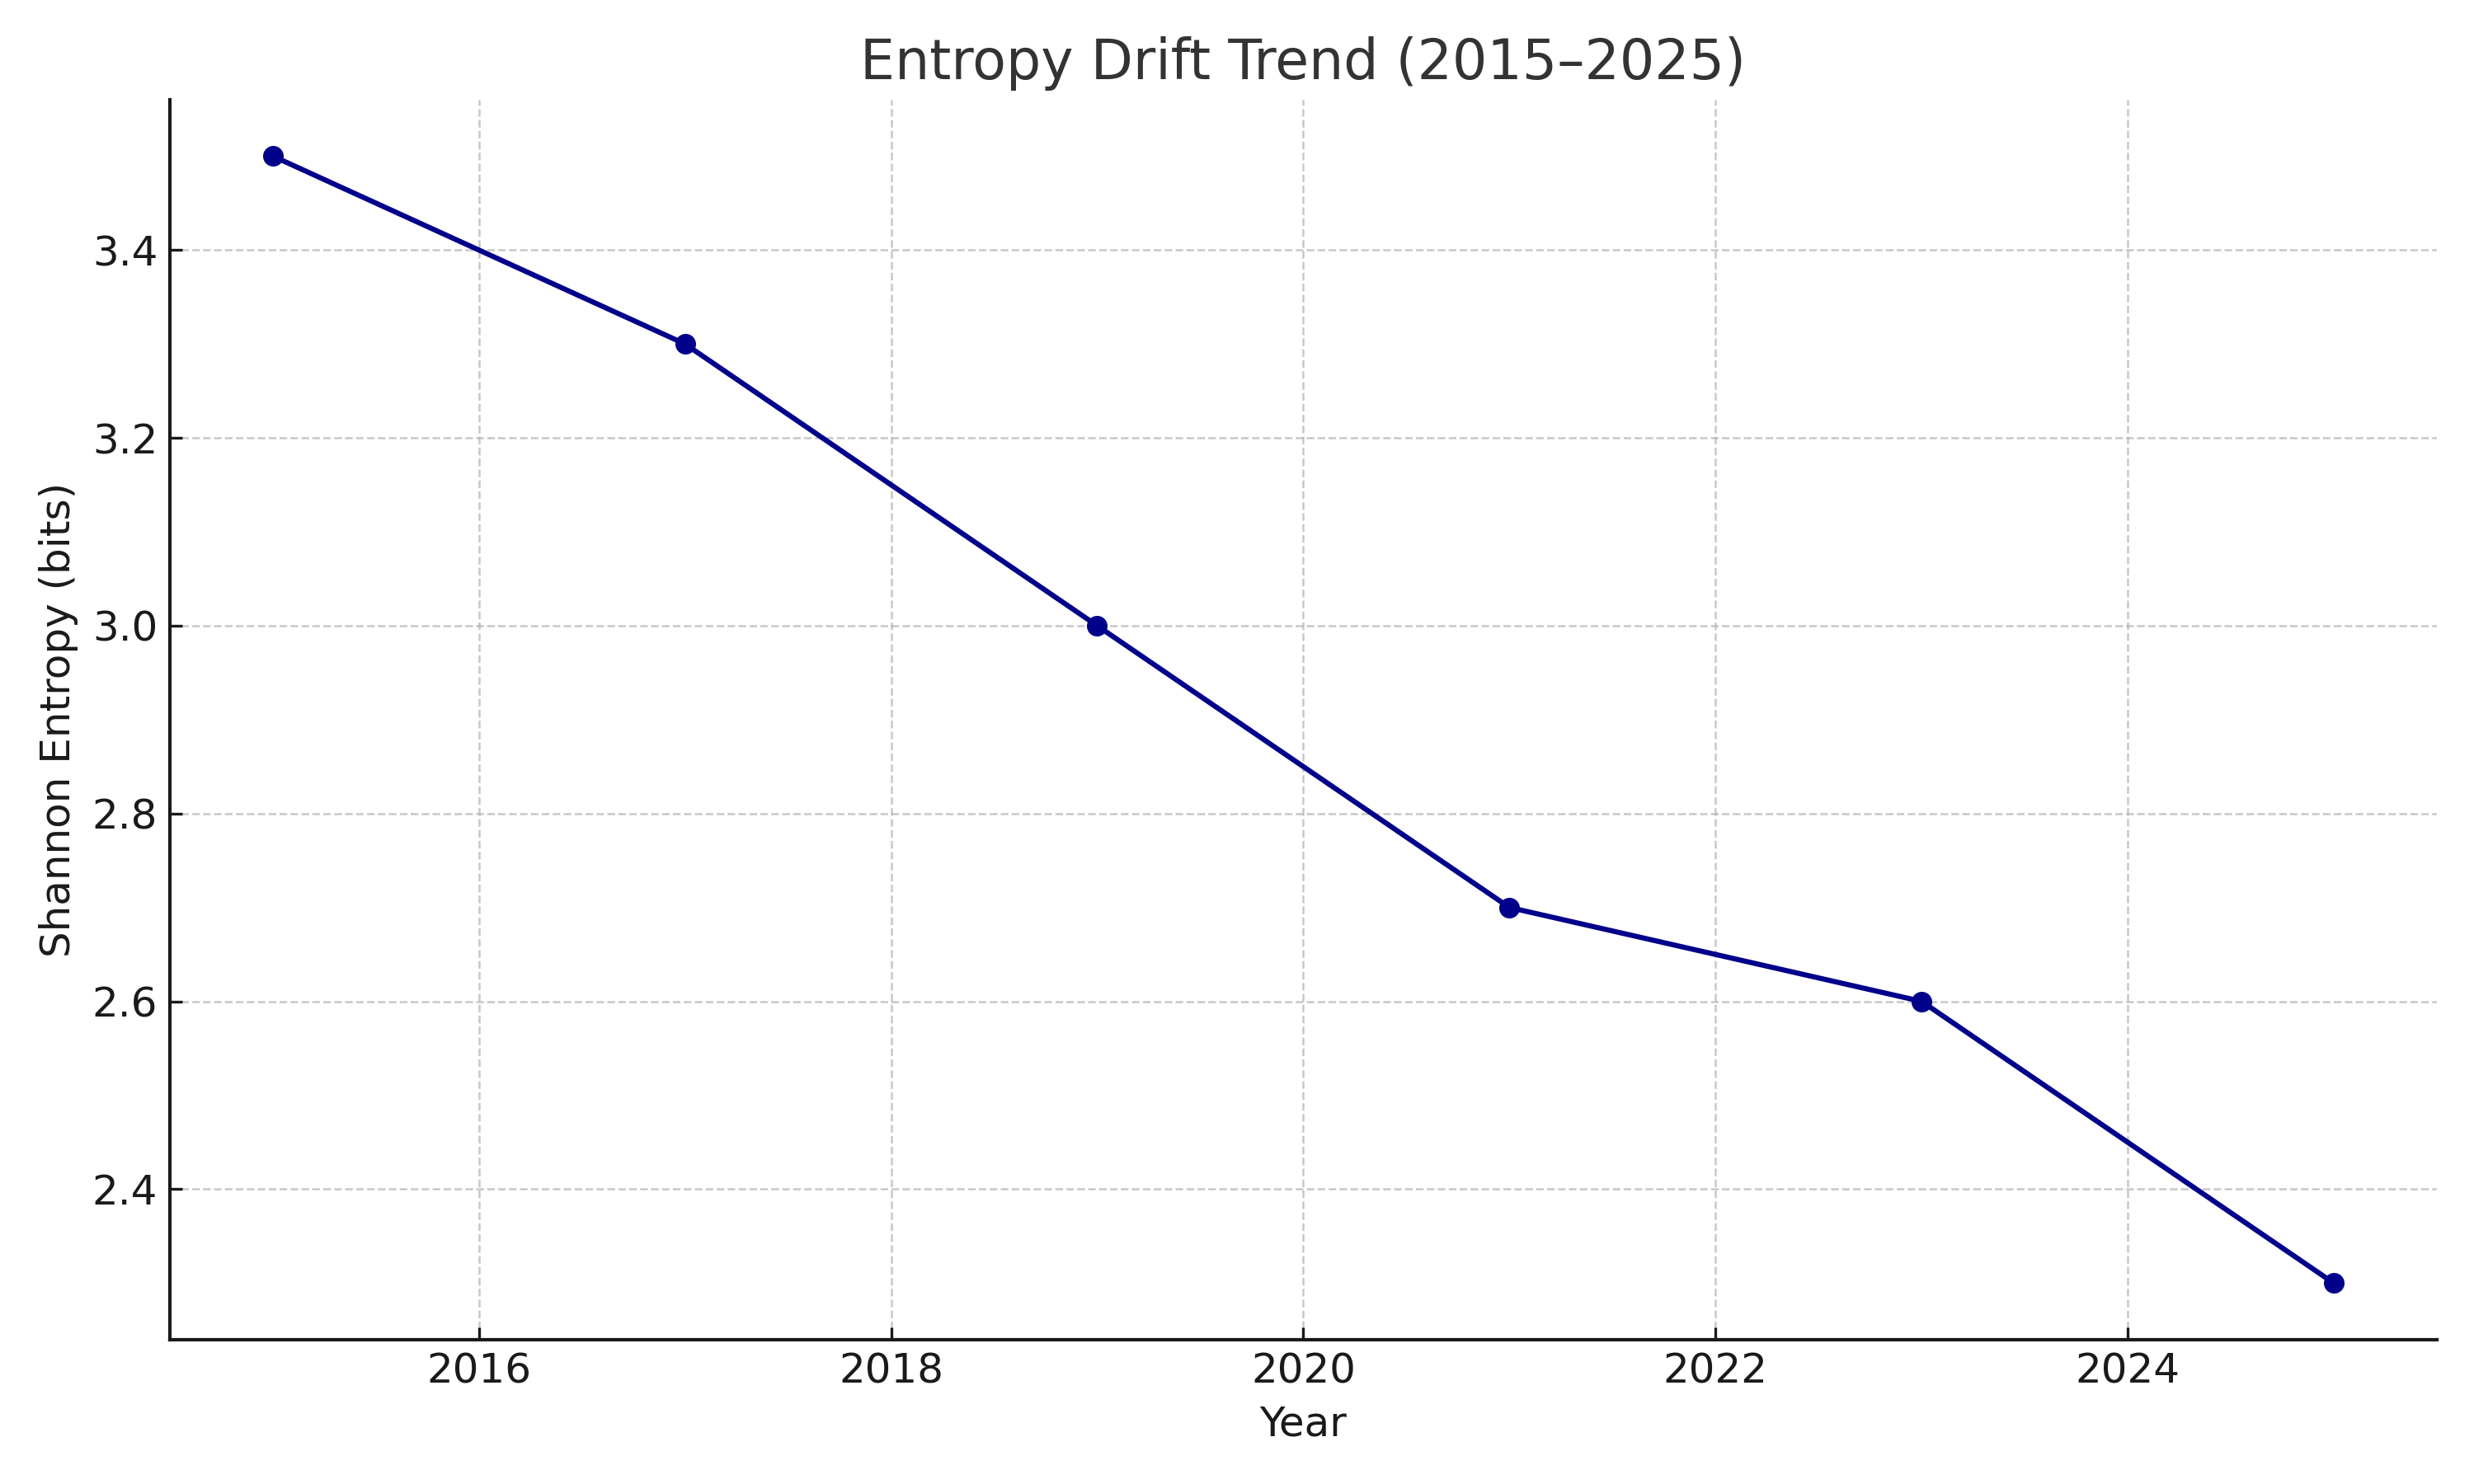
\includegraphics[width=0.95\linewidth]{assets/figures/entropy_drift_trend.png}
  \caption{\textbf{Entropy Drift (2015–2025)}: Contract entropy decline based on FPDS data for DHS, ICE, and Palantir-related procurements. Lower entropy corresponds with greater centralization and reduced systemic optionality.}
  \label{fig:entropy_drift}
\end{figure}

\section{Transition to the Collapse of Information Ecosystems}
\label{sec:transition_ch3}

The signal was clear: erasure wasn’t just happening through speech or policy—it was being funded, measured, and embedded. By the time I saw the 2025 contracts, I no longer needed a model to confirm the drift—I could feel it. And that realization carried me directly into the next layer of systemic unraveling: the collapse of information ecosystems themselves. Not just the patterns—but the very structures that once allowed us to detect them.

